\documentclass[12pt,a4paper,landscape]{article}
\usepackage{fontspec}
\usepackage[french]{babel}
\usepackage[utf8]{inputenc}
\usepackage[right=0.5cm, left=0.5cm,top=0.5cm,bottom=0.5cm]{geometry}
\usepackage{enumitem}
\usepackage{graphicx}
\usepackage{wrapfig}  % Package to wrap figures
\usepackage{array}
\usepackage{amsmath,amsfonts,amssymb,mathrsfs,amsthm}
\usepackage{fancyhdr}

\usepackage[usenames,svgnames,dvipsnames]{xcolor}
\usepackage{color}
%\mathchardef\times="2202
\definecolor{lightgray}{gray}{0.9}
\definecolor{ocre}{RGB}{0,244,244} 

\usepackage[most]{tcolorbox}
\usepackage{booktabs}
\usepackage[font={bf}]{caption}
\captionsetup[table]{box=colorbox,boxcolor=orange!20}
\usepackage{float}
\usepackage{esvect}
\usepackage{tabularx}
\usepackage{supertabular}
\usepackage{longtable}
\usepackage{colortbl}
\usepackage{fancybox}
\usepackage{tikz}
\usetikzlibrary{positioning,calc,intersections,patterns,decorations.pathmorphing,arrows.meta,decorations.markings}
\usetikzlibrary{arrows.meta}
\usepackage{ulem}
\usepackage{fontawesome5}
\usepackage{textcomp}
\usepackage{framed}
\usepackage{multicol}
\usepackage{varwidth}
\usetikzlibrary{calc}
\usepackage{pgfplots}
\usepackage{fourier}
\pgfplotsset{compat=1.11}
\usepackage{tkz-tab}
%\usepackage{xcolor}
\RequirePackage[framemethod=default]{mdframed}

\makeatletter
\tcbuselibrary{skins,breakable,xparse}
\tcbset{%
	save height/.code={%
		\tcbset{breakable}%
		\providecommand{#1}{2cm}%
		\def\tcb@split@start{%
			\tcb@breakat@init%
			\tcb@comp@h@page%
			\def\tcb@ch{%
				\tcbset{height=\tcb@h@page}%
				\tcbdimto#1{#1+\tcb@h@page-\tcb@natheight}%
				\immediate\write\@auxout{\string\gdef\string#1{#1}}%
				\tcb@ch%
			}%
			\tcb@drawcolorbox@standalone%
		}%
	}%
}

\makeatother
\newcommand{\oij}{$\left(\text{O};\vv{i},\vv{j},\vv{k}\right)$}
\colorlet{darkred}{red!30!black}
\newcommand{\red}[1]{\textcolor{darkred}{ #1}}
\newcommand{\rr}{\mathbb{R}}
\renewcommand{\baselinestretch}{1.2}
\setlength{\arrayrulewidth}{1.25pt}
\usepackage{titlesec}
\usepackage{titletoc}
\usepackage{minitoc}

%\usepackage[no-math]{fontspec}
\usepackage{polyglossia}
\makeatletter 
%\AtBeginDocument{\bidi@isloaded[]{frenchxetex}}
\makeatother
\setdefaultlanguage{french}
%\setdefaultlanguage[calendar=gregorian,locale=algeria]{arabic}
\setotherlanguage{english}
\newfontfamily\fontf[Scale=1]{Amiri-Bold.ttf} %Simplified Arabic
\newfontfamily\fontsf[Scale=1]{GE New Bold.ttf}%Aljazeera
\newfontfamily\myfont[Scale=1.3]{Bell MT}%AlBattar

%*************************************************************+
\colorlet{dlines}{orange!15!white}
\colorlet{llines}{orange!015!white}
\tikzset{
	dashed lines/.style={llines, very thin, densely dashed},
	strong lines/.style={dlines, very thin},
}
%--------------------------------------------------------------
\tcbset{
	enhanced,
	colback=white,
	boxrule=0.1pt,
	colframe=brown!10,
	fonttitle=\bfseries
}
\newcommand*{\arraycolor}[1]{\protect\leavevmode\color{#1}}
\newcolumntype{A}{>{\columncolor{blue!50!white}}c}
\newcolumntype{B}{>{\columncolor{LightGoldenrod}}c}
\newcolumntype{C}{>{\columncolor{FireBrick!50}}c}
\newcolumntype{D}{>{\columncolor{Gray!42}}c}
%------------------------------------------------
\newtcolorbox{box1}[2]{breakable,
	enhanced,
	leftrule=0pt,
	toprule=0pt,
	outer arc=0pt,
	arc=0pt,
	colframe=#2,
	colback=#2!3,title=#1,coltitle=white,
	attach boxed title to top right,
	boxed title style={
		colback=#2,
		outer arc=0pt,
		arc=0pt,
		top=3pt,
		bottom=3pt,
	},
	fonttitle= \bfseries}
\newtcolorbox{box2}[2]{enhanced,breakable,pad at break*=1mm,skin=enhancedlast jigsaw,
	attach boxed title to top right={xshift=4mm,yshift=-0.5mm},
	interior style={top color=#2!3!white,bottom color=white},
	boxed title style={empty,arc=0pt,outer arc=0pt,boxrule=0pt},
	underlay boxed title={
		\fill[#2] (title.north east) -- (title.north west)
		-- +(\tcboxedtitleheight-11.5mm,-\tcboxedtitleheight+1mm)
		-- ([xshift=-4mm,yshift=0.5mm]frame.north west) -- +(0mm,-1mm)
		-- (title.south east) -- cycle;
		\fill[#2!30!white!70!black] ([yshift=-0.5mm]frame.north west)
		-- +(-0.4,0) -- +(0,-0.3) -- cycle;
		\fill[#2!30!white!70!black] ([yshift=-0.5mm]frame.north east)
		-- +(0,-0.3) -- +(0.4,0) -- cycle; },
	colframe=#2,
	,title=#1,fonttitle= ,rightrule=1mm} 
\newtcolorbox{box3}[2]{enhanced,
	attach boxed title to top right={xshift=-0.3cm,yshift=-3mm},
	fonttitle= ,arc=10pt,sharp corners=uphill,
	colbacktitle=#2!45!white,coltitle=#2!10!black,colframe=#2!50!black,drop lifted shadow,
	interior style={top color=yellow!10!white,bottom color=#2!10!white},
	boxed title style={boxrule=0.75mm,colframe=#2!80!white,
		interior style={top color=#2!10!white,bottom color=#2!10!white,
			middle color=#2!50!white},
		drop fuzzy shadow},
	title=#1} 

%---------------------
\usepackage{chngcntr}
%\usepackage[inline,shortlabels]{enumitem}
\newcommand\tikzmark[1]{%
	\tikz[overlay,remember picture,baseline=-0.3ex] \coordinate (#1);}
\newcommand\catat[3][0pt]{%
	{\tikzmark{e}#2
		\begin{tikzpicture}[remember picture, overlay]
			\path let \p1 = (e), \p2 = (current page marginpar area.west) in node[yshift=-#1,text width=\marginparwidth,align=left,anchor=north west,font=\normalfont\small\color{RoyalBlue},inner ysep=0pt] at (\x2,\y1) {\tikzmark{s}\RaggedRight#3};
			\draw[RoyalBlue] let \p1 = (e), \p2 = (s) in (e) |- ([xshift=-5pt,yshift=0.5ex]s.west);
		\end{tikzpicture}%
	}%
}
%-------------------------
\definecolor{problemblue}{RGB}{100,134,158}
\definecolor{idiomsgreen}{RGB}{0,162,0}
\definecolor{exercisebgblue}{RGB}{192,232,252}
\tcbset{highlight math style={enhanced,
		colframe=red,colback=white,arc=0pt,boxrule=1pt}}
\newcounter{mbo}
\newtcolorbox[auto counter,number within=section,number freestyle={(\noexpand{\tcbcounter})}]{praproblem}{
	before title={\stepcounter{mbo}},
	breakable,
	enhanced,
	colback=white,
	boxrule=0pt,
	arc=0pt,
	outer arc=1pt,
	title=Théorème~(\thembo),
	fonttitle=\bfseries\sffamily\large\strut,
	coltitle=problemblue,
	colbacktitle=problemblue,
	title style={
		right color=white,
		left color=orange!80,
		middle color=orange!60
	},
	overlay={
		\draw[line width=1.5pt,problemblue] (title.north west) -- (title.north east);
	}
}
\newcounter{mtb}
\newtcolorbox[auto counter,number within=section,number freestyle={(\noexpand{\tcbcounter})}]{tcbexercise}{
	before title={\stepcounter{mtb}},
	breakable,
	enhanced,
	colback=white,
	boxrule=0pt,
	arc=0pt,
	outer arc=0pt,
	title=Exemple~(\themtb),
	fonttitle=\bfseries\sffamily\large\strut,
	coltitle=problemblue,
	colbacktitle=problemblue,
	title style={
		left color=exercisebgblue,
		right color=white,
		middle color=exercisebgblue  
	},
	overlay={
		\draw[line width=1.5pt,problemblue] (frame.south west) -- (frame.south east);
	}
}
%---------------------
%% this code comes from tColorbox Documentation Section 10.2.3 Page 153
\newtcolorbox{BoxRafa}[2][]
{enhanced,
	before skip=2mm,after skip=2mm,
	colback=yellow!20!white,colframe=black!50,boxrule=0.2mm,
	attach boxed title to top left =
	{xshift=0.6cm,yshift*=1mm-\tcboxedtitleheight},
	varwidth boxed title*=-1cm,
	boxed title style={frame code={
			\path[fill=green!30!black]
			([yshift=-1mm,xshift=-1mm]frame.north west)  
			arc[start angle=0,end angle=180,radius=1mm]
			([yshift=-1mm,xshift=1mm]frame.north east)
			arc[start angle=180,end angle=0,radius=1mm];
			\path[left color=green!60!black,right color = green!60!black,
			middle color = green!80!black]
			([xshift=-2mm]frame.north west) -- ([xshift=2mm]frame.north east)
			[rounded corners=1mm]-- ([xshift=1mm,yshift=-1mm]frame.north east) 
			-- (frame.south east) -- (frame.south west)
			-- ([xshift=-1mm,yshift=-1mm]frame.north west)
			[sharp corners]-- cycle;
		},interior engine=empty,
	},
	fonttitle=\bfseries\sffamily,
	title={#2},#1}
%---------------------
\usepackage{xpatch}

\xpatchcmd{\proof}{\itshape}{\bfseries\itshape}{}{}

\tcolorboxenvironment{proof}{
	blanker,
	before skip=\topsep,
	after skip=\topsep,
	borderline east={01pt}{1pt}{red},
	breakable,
	left=12pt,
	right=12pt, % I'd avoid this
}
%-------------------------
\begin{document}
%	\tikz[remember picture,overlay] {%
%		\draw [blue!10!black,line width=2mm]
%		(current page.south west)
%		rectangle (current page.north east)}
	\newcolumntype{Y}{>{\centering\arraybackslash}X}
	\tcbset{tab2/.style={enhanced,fonttitle=\bfseries,fontupper=\normalsize\sffamily,
			colback=white!10!white,breakable,colframe=red!50!black,colbacktitle=Salmon!40!white,
			coltitle=black,center title}}
	%===========================================
	\makeatletter
	\def\tcb@shadow@lifted#1#2#3#4{%
		\path[fill,rounded corners=\tcb@outer@arc,#4]
		([xshift=#1+#3,yshift=#2+#3]frame.south west)
		.. controls ([yshift=\dimexpr#3]frame.south) ..
		([xshift=-#1-#3,yshift=#2+#3]frame.south east)
		-- ([xshift=-#1-#3,yshift=#2-#3]frame.north east)
		-- ([xshift=#1+#3,yshift=#2-#3]frame.north west)
		-- cycle;
	}
	\tcbset{
		lifted shadow/.style args={#1#2#3#4}{shad@w app={%
				\begin{scope}[#4]%
					\tcb@shadow@lifted{#1}{#2}{\dimexpr-4\dimexpr#3}{opacity=0.01}%
					\tcb@shadow@lifted{#1}{#2}{\dimexpr-3\dimexpr#3}{opacity=0.02}%
					\tcb@shadow@lifted{#1}{#2}{\dimexpr-2\dimexpr#3}{opacity=0.04}%
					\tcb@shadow@lifted{#1}{#2}{\dimexpr-#3}{opacity=0.07}%
					\tcb@shadow@lifted{#1}{#2}{0pt}{opacity=0.11}%
					\tcb@shadow@lifted{#1}{#2}{\dimexpr+#3}{opacity=0.11}%
					\tcb@shadow@lifted{#1}{#2}{\dimexpr+2\dimexpr#3}{opacity=0.07}%
					\tcb@shadow@lifted{#1}{#2}{\dimexpr+3\dimexpr#3}{opacity=0.04}%
					\tcb@shadow@lifted{#1}{#2}{\dimexpr+4\dimexpr#3}{opacity=0.02}%
					\tcb@shadow@lifted{#1}{#2}{\dimexpr+5\dimexpr#3}{opacity=0.01}%
		\end{scope}}},%
		drop lifted shadow/.style={lifted shadow={1.5mm}{-1.5mm}{0.12mm}{#1}},
		drop lifted shadow/.default={black!50!white},%
		drop heavy lifted shadow/.style={lifted shadow={2mm}{-3mm}{0.16mm}{#1}},
		drop heavy lifted shadow/.default={black!50!white},%
	}
	\makeatother
	\newtcolorbox{boxone}{%
		enhanced,
		colback=black!0,
		boxrule=0pt,
		sharp corners,
		drop lifted shadow,
		frame hidden,
		fontupper=\bfseries,
		notitle,
		overlay={%
			\draw[Circle-Circle, gray!70!black, line width=2pt](frame.north west)--(frame.south west); 
			\draw[Circle-Circle, gray!70!black, line width=2pt](frame.north east)--(frame.south east);}
	}
	\newtcolorbox{boxtwo}{%
		enhanced,
		%frame style={draw=none},
		colback=gray!0,
		boxrule=0pt,
		sharp corners,
		drop lifted shadow,
		frame hidden,
		notitle,
		overlay={%
			\draw[{Triangle[right]}-{Triangle[left]}, , line width=2pt](frame.north west)--(frame.north east); 
			\draw[{Triangle[left]}-{Triangle[right]}, , line width=2pt](frame.south west)--(frame.south east);}
	}
	\newtcolorbox{boxthree}[2][]{%
		enhanced,
		breakable,
		drop fuzzy shadow southwest,
		%frame style={draw=none},
		colback=white,
		colbacktitle=orange!10,
		colback=orange!05!white,
		boxrule=0pt,
		fonttitle=\bfseries,
		coltitle=brown!30!black,
		sharp corners,
		frame hidden,
		title=#2,
		overlay={%
			\draw[thick, brown!70!black, double=orange, double distance=2pt] (frame.north west)--(frame.north east); 
			\draw[thick, brown!70!black, double=orange, double distance=2pt] (frame.south west)--(frame.south east);
			\fill[red!50!brown] ([shift={(3mm,.5mm)}]title.south west)--([shift={(-3mm,0mm)}]title.south east)--([shift={(3mm,-.5mm)}]title.south west)--cycle;}
	}
	%===========================================
	\textcolor{black}{\shadowbox{ plan N: 01 }}
	\hfill
	\textcolor{black}{\shadowbox{ \textbf{{\large CH1: Les Identités remarquables et puissances.}}}}
	\hfill  
	\textcolor{black}{\shadowbox{ Prof: {{ first_name }} {{ last_name }} }}
	\begin{boxone}
		\begin{multicols}{2} 
			\textcolor{black}{\myfont Lycée :  } {\sffamily  {{ school_name }}}
			\\
			\textcolor{black}{\myfont Année Scolaire  :} {\sffamily  \the\year{} - \the\numexpr\year+1\relax}
			\\
			\textcolor{black}{\myfont Période :} {\sffamily 10 heures.}
			\\
			%\textcolor{black}{\myfont Le jour   :} {\sffamily 21 mars 2022.}
			\\
			\textcolor{white}{.}\qquad\qquad\qquad\textcolor{black}{\myfont La classe :} {\sffamily 3APIC.}
			\\
			\textcolor{white}{.}\qquad\qquad\qquad\textcolor{black}{ \myfont Unité : } {\sffamily Le calcule numérique.}
			%			\\
			%			\textcolor{black}{\myfont Chapitre-1 :} {\sffamily Identités remarquables et puissances.}
		\end{multicols}
	\end{boxone}

	\begin{boxtwo}
		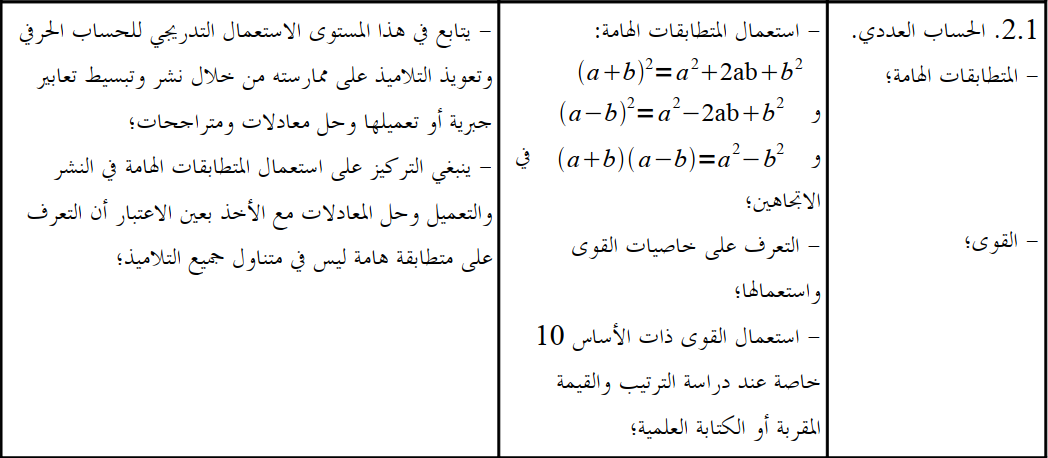
\includegraphics[width=\linewidth]{identités remarquables et puissances.png}	
		\textcolor{black}{\myfont\bfseries Les pré-requis :} Les 4 opérations sur les nombres rationnels, Calcul littéral, Développer et factoriser et simplifier des expressions algébriques, Identités remarquables sur les rationnels, Théorème de Pythagore.
		\\
		\textcolor{black}{\myfont\bfseries Les outils utilisés  :} Livre scolaire, Les ressources, les instructions pédagogiques.
	\end{boxtwo}\newpage
\renewcommand{\baselinestretch}{1.0}
	\begin{longtable}{|>{\centering\arraybackslash}p{3cm}|>{\raggedright\arraybackslash}p{5cm}|>{\raggedright\arraybackslash}p{13.5cm}|>{\raggedright\arraybackslash}p{5cm}|}
		\hline
		\rowcolor{black!20!white}\sffamily\textbf{OBJECTIFS}  &\sffamily\centering \textbf{ACTIVITÉS}
		& \sffamily\centering \textbf{CONTENU DE COURS} & \sffamily \textbf{APPLICATIONS}\\
		\hline 
		Développe et factorise une expression littérale\vspace*{4cm}
		
		Développe et factorise une expression littérale
		
		
		 & \colorbox{yellow!50!white}{\uline{\sffamily \textbf{Activité-1 :} }}\par%\bigskip
		\begin{enumerate}
			\item Développé et réduis :
			
			(i) $x(2x+1)$
			
			(ii) $5x^2(x+7)$ 
			
			(ii) $a(c+d)+b(c+d)$
			
			\item Factoriser :
			
			(i) $15b - 15c$
			
			(ii) $10a + 5c$ 
			
			(iii) $a(c+d)+b(c+d)$
			
		\end{enumerate}
		\colorbox{yellow!50!white}{\uline{\sffamily \textbf{Activité-2 :} }}\par%\bigskip
			ABCD est un rectangle
		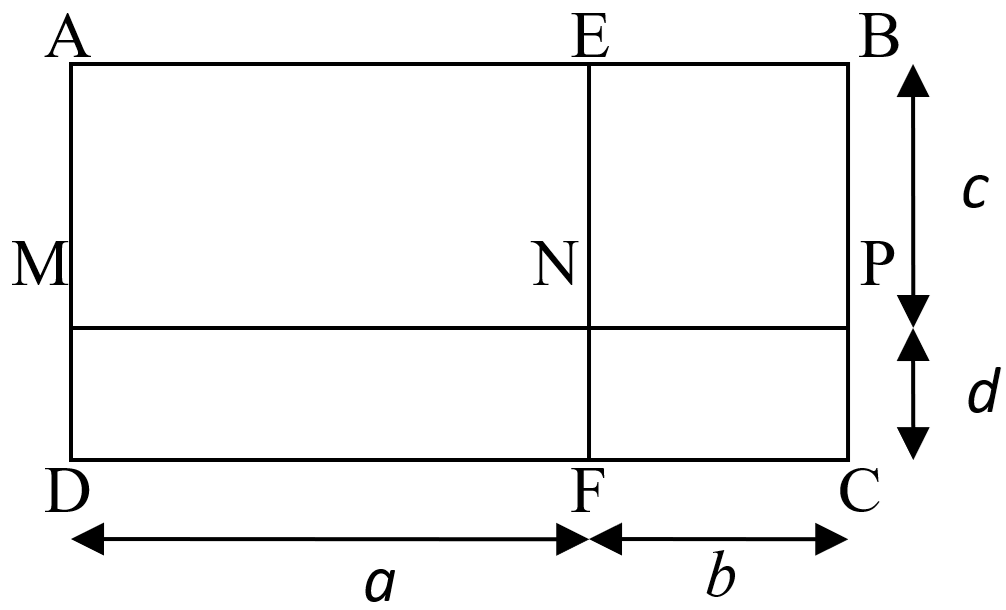
\includegraphics[width=5cm]{z.png}
		
		Calculer de 2 méthodes l'aire du rectangle ABCD et déduire que :
		\[ (a + b)(c + d) = ac + ad + bc + bd \]
		& 
		%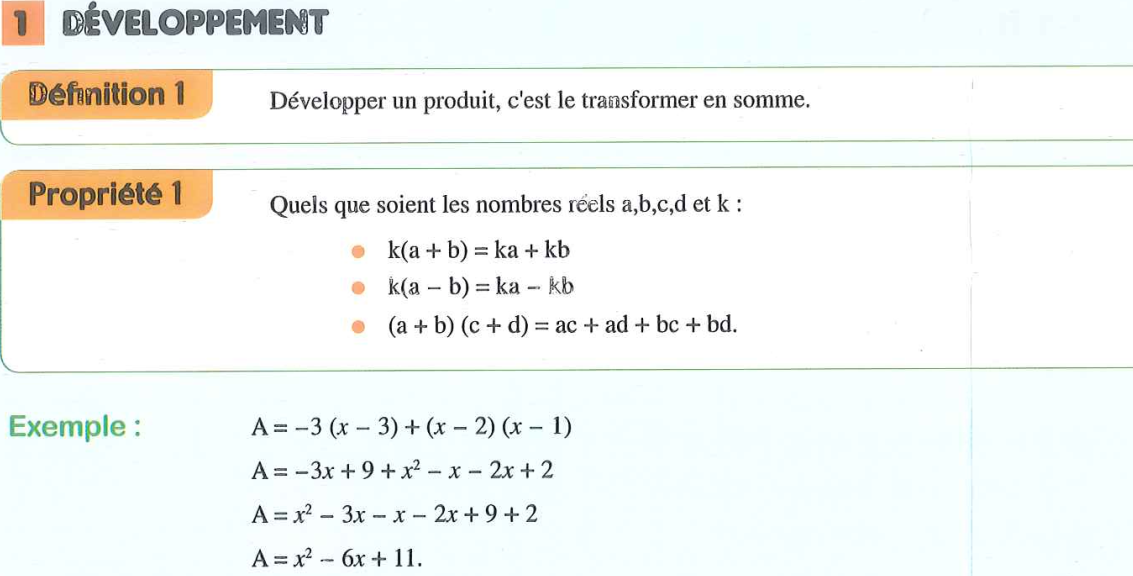
\includegraphics[width=\linewidth]{1.png}	
		\textcolor{Red}{\uline{\sffamily \textbf{I. Développement et Factorisation :} }}\par
		\textcolor{Green}{\uline{\sffamily \textbf{1- Définition:} }}\par
		\begin{BoxRafa}[colbacktitle = green]{Définition}
			\textbf{Développer} un produit signifie le transformer en une \textbf{somme algébrique}
			
			\textbf{Factoriser} une somme signifie le transformer en un  \textbf{produit algébrique}.
		\end{BoxRafa}
		\textcolor{Green}{\uline{\sffamily \textbf{2- Propriétés:} }}\par
		\begin{BoxRafa}[colbacktitle = green]{Propriété-1}
			$a$, $b$ et $k$ sont des nombres rationnels. On a:\vspace*{.5cm}
			
			\tcbhighmath[boxrule=0.3pt,colframe=red,drop fuzzy shadow=red]{$ k(a + b) = ka + kb $} \qquad ,\qquad \tcbhighmath[boxrule=0.3pt,colframe=red,drop fuzzy shadow=red]{$ k(a - b) = ka - kb $ }
		\end{BoxRafa}
		\begin{BoxRafa}[colbacktitle = Orange]{Exemples-1:}
			Développement des expressions:
			
			$ 3(5a+7) = 3\times5a + 3\times7 = 15a + 21 $
			
			$ 2x(3x+2) = 2x\times3x + 2x\times2 = 6x^2 + 4x $
			
		\end{BoxRafa}
		\begin{BoxRafa}[colbacktitle = green]{Propriété-2}
			$a$, $b$, $c$, $d$ sont des nombres rationnels. On a:\vspace*{.5cm}
			
			\qquad \tcbhighmath[boxrule=0.3pt,colframe=red,drop fuzzy shadow=red]{$ (a + b)(c + d) = ac + ad + bc + bd $ }
		\end{BoxRafa}
		\begin{BoxRafa}[colbacktitle = Orange]{Exemples-2:}
			Développement des expressions :
			
			$ (2x - 1)(x - 2) = 2x\times x - 2x\times2 -1\times x -1\times(-2) = 2x^2 - 4x - x + 2 = 2x^2-5x+2 $
			
		\end{BoxRafa}
		& \colorbox{yellow!50!white}{\uline{\sffamily \textbf{Exercice-1:} }}\par
		Développer puis simplifier les expressions suivantes :
		$\begin{aligned}
			&a=2(1-2x)+3(x-1) \\
			&b=(2x^2-6)(x^2+4) \\
			&c=7x(3x-5)+(3x-5)(x-1) \\
			&d=(8x^3-2x+1)(x+3) \\
			&e=(x+y+z)(x+y-z)
		\end{aligned}$
		\\ \hline
		Factoriser des expressions avec un facteur commun	&	&
		\textcolor{Red}{\uline{\sffamily \textbf{II. Factorisation:} }}\par
		\begin{BoxRafa}[colbacktitle = green]{Définition}
			\textbf{Factoriser} une somme signifie la transformer en \textbf{produit}.
		\end{BoxRafa}
		\begin{BoxRafa}[colbacktitle = green]{Règle}
			$a$, $b$ et $k$ sont des nombres rationnels. On a:%\vspace*{.5cm}
			
			\tcbhighmath[boxrule=0.3pt,colframe=red,drop fuzzy shadow=red]{$ ka + kb = k(a + b) $} \qquad ,\qquad \tcbhighmath[boxrule=0.3pt,colframe=red,drop fuzzy shadow=red]{$ ka - kb = k(a - b) $ }
		\end{BoxRafa}
		\begin{BoxRafa}[colbacktitle = Orange]{Exemples-1:}
			Factorisation des expressions:
			
			$\begin{aligned}
				&4a^{2}+3a=4\times a\times a+3\times a=a(4a+3)\\
				&(x+7)(5-4x)-2(5-4x)=(5-4x)\times(x+7-2)=(5-4x)(x+5)\\
				&(x+3)^{2}+(x+4)(x+3)=(x+3)(x+3+x+4)=(x+3)(2x+7)
			\end{aligned}$
			
		\end{BoxRafa}
		& \colorbox{yellow!50!white}{\uline{\sffamily \textbf{Exercice-2:} }}\par
		Factoriser les expressions:
		$\begin{aligned}
			&\text{25x-15} \\
			&\text{5x-3} \\
			&(3x+1)^{2}-(3x+1)(2x+5) \\
			&7x(2x-9)-11(9-2x) \\
			&6x^{2}+12x+6 \\
			&xy-x-y+1
		\end{aligned}$
			\\ \hline
		
		Connaitre les identités remarquables &	
		\colorbox{yellow!50!white}{\uline{\sffamily \textbf{Activité-3 :} }}\par%\bigskip
		
		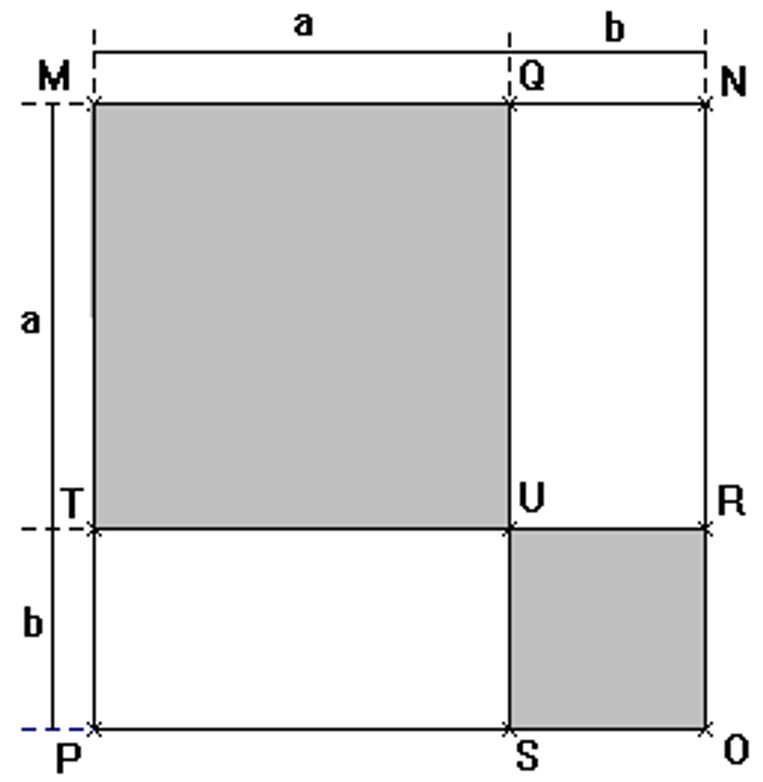
\includegraphics[width=4cm]{t.png}
		
			1) Calculer l'aire du carre $MNPQ$ de deux façons différentes et déduire que : $\left(a+b\right)^2 = a^2+2ab+b^2$
			
			2) Déduire que : $(a-b)^2=a^2-2ab+b^2$
			
			(On remarque que : $a-b =a+(-b)$)
			& 	
			\textcolor{Red}{\uline{\sffamily \textbf{III. Identités remarquables:} }}\par
			\textcolor{Green}{\uline{\sffamily \textbf{1- Carré d'une somme:} }}\par
		\begin{BoxRafa}[colbacktitle = green]{Propriété}
			$a$ et $b$ sont des nombres rationnels. On a:%\vspace*{.5cm}
			
			\begin{tikzpicture}[
				roundnode/.style={circle, draw=green!60, fill=green!5, very thick, minimum size=7mm},
				squarednode/.style={rectangle, draw=red!60, fill=red!5, very thick, minimum size=5mm},
				]
				%Nodes
				\node[squarednode]      (maintopic)                              {$\left(a+b\right)^2$};
				\node[roundnode]        (uppercircle)       [right=of maintopic] {=};
				\node[squarednode]      (rightsquare)       [right=of uppercircle] {$a^2+2ab+b^2$};
				%\node[roundnode]        (lowercircle)       [below=of maintopic] {4};
				
				%Lines
				%\draw[->] (uppercircle.south) -- (maintopic.north);
				\draw[->] (maintopic.north) .. controls +(up:7mm) and +(right:0mm) .. (rightsquare.north);
				\draw[->] (rightsquare.south) .. controls +(down:7mm) and +(right:0mm) .. (maintopic.south);
				%\draw[->] (rightsquare.south) .. controls +(down:7mm) and +(right:7mm) .. (lowercircle.east);
			\end{tikzpicture}
		\end{BoxRafa}
		\begin{BoxRafa}[colbacktitle = Orange]{Exemples-1:}
			
			$\begin{aligned}
				&(2\mathrm{x}+3)^2=(2\mathrm{x})^2+2\times2\mathrm{x}\times3+3^2=4\mathrm{x}^2+12\mathrm{x}+9 \\
				&16\mathrm{x}^2+8\mathrm{x}+1=(4\mathrm{x}+1)^2 \\
				&25\mathrm{x}^2+20\mathrm{x}+4=(5\mathrm{x}+2)^2
			\end{aligned}$
			
		\end{BoxRafa}&
		\colorbox{yellow!50!white}{\uline{\sffamily \textbf{Exercice-3:}}}\par
		1) Développer puis simplifier les expressions suivantes :
		
		$\begin{aligned}
			&A=\left(9x+8\right)^2 \\ &B=\left(6+5x\right)^2 
		\end{aligned}$
		
		2) Factoriser :
		$\begin{aligned}
			&\mathbf{C}=x^2+8x+16\\
			&\text{D=49}x^2+42x+9+\mathrm{x}(7x+3)
		\end{aligned}$
		
		3) On considère $F = (2x + 3)^2 + (2x + 3)( x- 1)$.
		
		a. Développer et réduire $F$.
		
		b. Factoriser $F$.
		
		c. Calculer $F$ Pour $x=-\dfrac{2}{3}$ .
		
		\\
		\hline
		Connaitre les identités remarquables
		&
		\colorbox{yellow!50!white}{\uline{\sffamily \textbf{Activité-4 :} }}\par%\bigskip
		$a$ et $b$ deux nombres réels
		
		Développer et réduire : $\left( a-b\right) \left( a+b\right) $
		
		&
		\textcolor{Green}{\uline{\sffamily \textbf{2- Carré d'une différence:} }}\par
		\begin{BoxRafa}[colbacktitle = green]{Propriété}
			$a$ et $b$ sont des nombres rationnels. On a:%\vspace*{.5cm}
			
			\begin{tikzpicture}[
				roundnode/.style={circle, draw=green!60, fill=green!5, very thick, minimum size=7mm},
				squarednode/.style={rectangle, draw=red!60, fill=red!5, very thick, minimum size=5mm},
				]
				%Nodes
				\node[squarednode]      (maintopic)                              {$\left(a-b\right)^2$};
				\node[roundnode]        (uppercircle)       [right=of maintopic] {=};
				\node[squarednode]      (rightsquare)       [right=of uppercircle] {$a^2-2ab+b^2$};
				%\node[roundnode]        (lowercircle)       [below=of maintopic] {4};
				
				%Lines
				%\draw[->] (uppercircle.south) -- (maintopic.north);
				\draw[->] (maintopic.north) .. controls +(up:7mm) and +(right:0mm) .. (rightsquare.north);
				\draw[->] (rightsquare.south) .. controls +(down:7mm) and +(right:0mm) .. (maintopic.south);
				%\draw[->] (rightsquare.south) .. controls +(down:7mm) and +(right:7mm) .. (lowercircle.east);
			\end{tikzpicture}
		\end{BoxRafa}
		\begin{BoxRafa}[colbacktitle = Orange]{Exemples-1:}
			
			$\begin{aligned}
				&(2x-3)^{2}=(2x)^{2}-2\times2x\times3+3^{2}=4x^{2}-12x+9 \\
				&99^{2}=(100-1)^{2}=100^{2}-2\times100\times1+1^{2}=1000-200+1=9801 \\
				&16x^{2}-8x+1=(4x-1)^{2}
			\end{aligned}$
			
		\end{BoxRafa}
		\textcolor{Green}{\uline{\sffamily \textbf{3- Carré d'une différence:} }}\par
		\begin{BoxRafa}[colbacktitle = green]{Propriété}
			$a$ et $b$ sont des nombres rationnels. On a:%\vspace*{.5cm}
			
			\begin{tikzpicture}[
				roundnode/.style={circle, draw=green!60, fill=green!5, very thick, minimum size=7mm},
				squarednode/.style={rectangle, draw=red!60, fill=red!5, very thick, minimum size=5mm},
				]
				%Nodes
				\node[squarednode]      (maintopic)                              {$\left(a+b\right)\left(a-b\right)$};
				\node[roundnode]        (uppercircle)       [right=of maintopic] {=};
				\node[squarednode]      (rightsquare)       [right=of uppercircle] {$a^2-b^2$};
				%\node[roundnode]        (lowercircle)       [below=of maintopic] {4};
				
				%Lines
				%\draw[->] (uppercircle.south) -- (maintopic.north);
				\draw[->] (maintopic.north) .. controls +(up:7mm) and +(right:0mm) .. (rightsquare.north);
				\draw[->] (rightsquare.south) .. controls +(down:7mm) and +(right:0mm) .. (maintopic.south);
				%\draw[->] (rightsquare.south) .. controls +(down:7mm) and +(right:7mm) .. (lowercircle.east);
			\end{tikzpicture}
		\end{BoxRafa}
		\begin{BoxRafa}[colbacktitle = Orange]{Exemples-1:}
			
			$\begin{aligned}
				&(2x+3)(2x-3)=(2x)^{2}-3^{2}=4x^{2}-9 \\
				&99\times101=(100+1)(100-1)=100^{2}-1^{2}=10000-1=9999 \\
				&16x^{2}-9=(4x+3)(4x-3) \\
				&\left(\sqrt{11}+\sqrt{7}\right)\left(\sqrt{11}-\sqrt{7}\right)=\sqrt{11}^{2}-\sqrt{7}^{2}=11-7=4
			\end{aligned}$
			
		\end{BoxRafa}
		&
		\colorbox{yellow!50!white}{\uline{\sffamily \textbf{Exercice-4:}}}\par
		1) Développer puis simplifier les expressions suivantes :
			$$X=\left(\frac{x}{2}-2\right)^{2} \quad Y=\left(\frac{2}{3}x-\frac{3}{5}\right)^{2}$$
		2) Factoriser :

		$$\begin{aligned}
			&Z=9x^{2}-24x+16\\
			&W=25x^{2}+9-30x
		\end{aligned}$$
		
		\colorbox{yellow!50!white}{\uline{\sffamily \textbf{Exercice-5:}}}\par
		1)	Développer $A(x) = (2x + 1) (2x -1)$.
		
		2)	Calculer $A(x)$ pour $x =\sqrt{5}$
		
		3)	Factoriser $B(x)=9x^2-16$
		
		\colorbox{yellow!50!white}{\uline{\sffamily \textbf{Exercice-6:}}}\par
		Calculer mentalement : $78\times82 \quad ; \quad592-61^2$
		
		\\ \hline
		 &	
		\colorbox{yellow!50!white}{\uline{\sffamily \textbf{Activité-5 :} }}\par%\bigskip
		
		1) Calculer les puissances suivantes: 
		$$\begin{aligned}
			&\left(\frac{2}{3}\right)^{3}\quad;\quad\left(-5\right)^{4}\quad;\left(\frac{2}{3}\right)^{1}\\
			&\left(-54.7\right)^{0}\quad;\quad1^{12}\quad;\quad0^{12}\\
			&\left(-1\right)^{4}\ ;\ \left(-1\right)^{7}\ ;\-1^{4}\ ;\ -1^{7}
		\end{aligned}$$
		
		2) Calculer les puissances suivantes:
		
		$5^{- 2}$ ; $1^{- 12}$ ; $10^{- 3}$
		
		$\left ( \frac 23\right ) ^{- 3}$ ; $\left ( - 5\right ) ^4$ $; \left ( \frac 23\right ) ^{- 1}$
		& 	
		\textcolor{Red}{\uline{\sffamily \textbf{IV. Puissance d’un nombre réel} }}\par
		%\textcolor{Green}{\uline{\sffamily \textbf{1- Carré d'une somme:} }}\par
		\begin{BoxRafa}[colbacktitle = green]{Définition:}
			Soit $a$ un nombre quelconque et $m$ un entier naturel non nul. On note   $a^m$ le nombre défini par : %\vspace*{.5cm}
			
			\hspace*{3cm}\begin{tikzpicture}[
				roundnode/.style={circle, draw=green!60, fill=green!5, very thick, minimum size=7mm},
				squarednode/.style={rectangle, draw=red!60, fill=red!5, very thick, minimum size=5mm},
				]
				%Nodes
				\node[squarednode]	(maintopic)	{$a^m=\underbrace{a\times a\times\cdots\times a}_{m\ fois}$};
				%\node[roundnode]        (uppercircle)       [right=of maintopic] {=};
				%\node[squarednode]      (rightsquare)       [right=of uppercircle] {$a^2+2ab+b^2$};
				%\node[roundnode]        (lowercircle)       [below=of maintopic] {4};
				
				%Lines
				%\draw[->] (uppercircle.south) -- (maintopic.north);
				%\draw[->] (maintopic.north) .. controls +(up:7mm) and +(right:0mm) .. (rightsquare.north);
				%\draw[->] (rightsquare.south) .. controls +(down:7mm) and +(right:0mm) .. (maintopic.south);
				%\draw[->] (rightsquare.south) .. controls +(down:7mm) and +(right:7mm) .. (lowercircle.east);
			\end{tikzpicture}\vspace{-.3cm}
			\begin{itemize}
				\item[$\blacktriangleright$]  Le nombre $a^m$ est le produit du nombre $a$ par lui-même $m$ fois.
				\item[$\blacktriangleright$]  Le nombre $a^m$ se lit "\textbf{a puissance m}" ou "\textbf{a exposant m}".
				\item[$\blacktriangleright$]  Par convention on admet que $a^0=1$
			\end{itemize}
		\end{BoxRafa}
		\begin{BoxRafa}[colbacktitle = Orange]{Remarques:}
			
			\begin{itemize}
				\item[$\blacktriangleright$]  Le nombre $\mathbf{a^{2}}$ se lit aussi "\textbf{a au carré}" ; et le nombre $\mathbf{a^{3}}$ se lit aussi "\textbf{a au cube}".
				\item[$\blacktriangleright$]  On a toujours $\mathbf{a^{1}=a}$ (donc si un nombre est écrit sans puissance, on considère qu’il est à la puissance 1).
				\item[$\blacktriangleright$]  $a^{-n}$ est \textbf{l’inverse} de $a^{n}$
			\end{itemize}
			
		\end{BoxRafa}
		\begin{BoxRafa}[colbacktitle = Orange]{Exemples:}
			
			\begin{itemize}
				\item[$\blacktriangleright$]  $2^{3}=2\times2\times2$.
				\item[$\blacktriangleright$]  On a $3^7=\underbrace{3\times3\times3\times3\times3\times3\times3}_{7facteurs}$.
				\item[$\blacktriangleright$]  On a aussi $5\times5\times5\times5\times5\times5\times5\times5\times5\times5=5^{10}$ (le nombre de 5 qui se multiplient est 10).
			\end{itemize}
			
		\end{BoxRafa}
		\begin{BoxRafa}[colbacktitle = Orange]{MISE EN GARDE:}
			
			$\blacktriangleright$ Il ne faudra pas confondre le nombre $\mathbf{a^{m}}$ avec $\mathbf{a\times m}$
			
			$\blacktriangleright$ Par exemple $2^{3}=2\times2\times2=8$ ; alors que $2\times3=6$ (On voit bien que les résultats sont différents).
			
			
		\end{BoxRafa}
		&
		\colorbox{yellow!50!white}{\uline{\sffamily \textbf{Exercice-7:}}}\par
		Calculer les puissances suivantes :
		
		$\begin{aligned}
			&a=\left(-4\right)^{4}\quad b=\left(3\sqrt{2}\right)^{2} \\
			&c=\left(-\sqrt{2}\right)^{3}d=\left(\sqrt{2}\right)^{4} \\
			&e=\left({\frac{-4}{5}}\right)^{4}\quad f=\left({\frac{-4}{5}}\right)^{-1} \\
			&j=(2^{2}+3^{-2})^{-1} \\
			&h=\left[((\frac{4}{\sqrt{5}})^{-1}\times(\frac{-1}{2})^{2})^{-2}\right]
		\end{aligned}$
		\\
		\hline
		&	
		\colorbox{yellow!50!white}{\uline{\sffamily \textbf{Activité-6 :} }}\par%\bigskip
		
		Simplifier les expressions suivantes : 
		
		$\begin{aligned}
			&A=\left(\sqrt{2}\right)^{3}\times\left(\sqrt{2}\right)^{5}\times\left(\sqrt{2}\right) \\
			&B=\left(\sqrt{3}\right)^{-3}\times\left(\sqrt{3}\right)^{5} \\
			&C=\left(\sqrt{3}\right)^{2}\times5^{2} \\
			&D=\left(\left(\sqrt{3}\right)^{2}\right)^{3} \\
			&E=\frac{\left(\sqrt{3}\right)^{5}}{\left(\sqrt{3}\right)^{3}}
		\end{aligned}$
		& 	
		\textcolor{Red}{\uline{\sffamily \textbf{V. Propriétés des puissances} }}\par
		%\textcolor{Green}{\uline{\sffamily \textbf{1- Carré d'une somme:} }}\par
		{Les puissances ont des propriétés spécifiques permettant des calculs rapides.}
		\begin{BoxRafa}[colbacktitle = green]{RÈGLE N$^\circ$1:(Produit De Deux Puissances)}
			\hspace*{2cm}\begin{tikzpicture}[
				roundnode/.style={circle, draw=green!60, fill=green!5, very thick, minimum size=7mm},
				squarednode/.style={rectangle, draw=red!60, fill=red!5, very thick, minimum size=5mm},
				]
				%Nodes
				\node[squarednode]	(maintopic)	{$\underbrace{\qquad a^m\times a^p\qquad}_{\text{C'est le même nombre}}=\underbrace{\quad\qquad a^{m+p}\quad\qquad}_{\text{On additionne les puissances}}$};
				%\node[roundnode]        (uppercircle)       [right=of maintopic] {=};
				%\node[squarednode]      (rightsquare)       [right=of uppercircle] {$a^2+2ab+b^2$};
				%\node[roundnode]        (lowercircle)       [below=of maintopic] {4};
				
				%Lines
				%\draw[->] (uppercircle.south) -- (maintopic.north);
				%\draw[->] (maintopic.north) .. controls +(up:7mm) and +(right:0mm) .. (rightsquare.north);
				%\draw[->] (rightsquare.south) .. controls +(down:7mm) and +(right:0mm) .. (maintopic.south);
				%\draw[->] (rightsquare.south) .. controls +(down:7mm) and +(right:7mm) .. (lowercircle.east);
			\end{tikzpicture}\vspace{-.1cm}
		\end{BoxRafa}
		
		\begin{BoxRafa}[colbacktitle = Orange]{Exemples:}
			
			\textbf{Calculons les nombres $x=\frac{5^8}{5^6}$ et $y=\frac{3^{14}}{3^8}$ en donnant les résultats sous forme de puissances.}
			
			On applique directement la règle qui nous donne : $x=3^{4}\times3^{2}=\underbrace{\qquad\qquad 3^{4+2}\qquad\qquad}_{\text{On additionne les puissances}}=3^{6}$ et de même $y=7^3\times7^2=7^{3+2}=7^5$
			
		\end{BoxRafa}
		\begin{BoxRafa}[colbacktitle = green]{RÈGLE N$^\circ$2:(Quotient De Deux Puissances)}
			\hspace*{1.5cm}\begin{tikzpicture}[
				roundnode/.style={circle, draw=green!60, fill=green!5, very thick, minimum size=7mm},
				squarednode/.style={rectangle, draw=red!60, fill=red!5, very thick, minimum size=5mm},
				]
				%Nodes
				\node[squarednode]	(maintopic)	{$\underbrace{\qquad\qquad\frac{a^m}{a^p}\qquad\qquad}_{\text{C'est le même nombre }a}=\underbrace{\qquad\qquad a^{m-p}\qquad\qquad}_{\text{On soustrait les puissances}}$};
				%\node[roundnode]        (uppercircle)       [right=of maintopic] {=};
				%\node[squarednode]      (rightsquare)       [right=of uppercircle] {$a^2+2ab+b^2$};
				%\node[roundnode]        (lowercircle)       [below=of maintopic] {4};
				
				%Lines
				%\draw[->] (uppercircle.south) -- (maintopic.north);
				%\draw[->] (maintopic.north) .. controls +(up:7mm) and +(right:0mm) .. (rightsquare.north);
				%\draw[->] (rightsquare.south) .. controls +(down:7mm) and +(right:0mm) .. (maintopic.south);
				%\draw[->] (rightsquare.south) .. controls +(down:7mm) and +(right:7mm) .. (lowercircle.east);
			\end{tikzpicture}\vspace{-.1cm}
		\end{BoxRafa}
		
		\begin{BoxRafa}[colbacktitle = Orange]{Exemples:}
			\textbf{Calculons les nombres $x=3^4\times3^2$ et $y=7^{3}\times7^{2}$ en donnant les résultats sous forme de puissances.}
			
			La règle nous donne directement: $x=\frac{5^{8}}{5^{6}}=\underbrace{\quad\qquad5^{8-6}\quad\qquad}_{\text{On soustrait les puissances}}=5^{2}$ 
			
			Et de même $y=\frac{3^{14}}{3^8}=3^{14-8}=3^6$
			
		\end{BoxRafa}
		\begin{BoxRafa}[colbacktitle = green]{RÈGLE N$^\circ$3:(Puissance D’une Puissance)}
			\hspace*{1.5cm}\begin{tikzpicture}[
				roundnode/.style={circle, draw=green!60, fill=green!5, very thick, minimum size=7mm},
				squarednode/.style={rectangle, draw=red!60, fill=red!5, very thick, minimum size=5mm},
				]
				%Nodes
				\node[squarednode]	(maintopic)	{$\underbrace{\qquad\qquad\qquad\left(a^m\right)^p\qquad\qquad\qquad}_{\text{On éléve une puissance à une autre puissance}}=\underbrace{\quad\qquad a^{m\times p}\qquad\quad}_{\text{On multiplie les puissances}}$};
				%\node[roundnode]        (uppercircle)       [right=of maintopic] {=};
				%\node[squarednode]      (rightsquare)       [right=of uppercircle] {$a^2+2ab+b^2$};
				%\node[roundnode]        (lowercircle)       [below=of maintopic] {4};
				
				%Lines
				%\draw[->] (uppercircle.south) -- (maintopic.north);
				%\draw[->] (maintopic.north) .. controls +(up:7mm) and +(right:0mm) .. (rightsquare.north);
				%\draw[->] (rightsquare.south) .. controls +(down:7mm) and +(right:0mm) .. (maintopic.south);
				%\draw[->] (rightsquare.south) .. controls +(down:7mm) and +(right:7mm) .. (lowercircle.east);
			\end{tikzpicture}\vspace{-.1cm}
		\end{BoxRafa}
	
		&
		\colorbox{yellow!50!white}{\uline{\sffamily \textbf{Exercice-8:}}}\par
		Simplifier les expressions suivantes :
		
		$\begin{aligned}&\left(\sqrt{7}\right)^{-13}\times\left(\sqrt{7}\right)^{65}\\&\left(\sqrt{3}\right)^{6}\times\left(\sqrt{3}\right)^{-5}\times\left(\sqrt{3}\right)\end{aligned}$
		\colorbox{yellow!50!white}{\uline{\sffamily \textbf{Exercice-9:}}}\par
		Simplifier les expressions suivantes :
		
		$\begin{aligned}
			&a= (-4)^{3}\times(-4)^{12} \\
			&b=5^{6}\times(\sqrt{2})^{6}  \\
			&c= \frac{(-\sqrt{2})^{3}}{(-\sqrt{2})^{-8}} \\
			&d=\left(\sqrt{2}^{5}\right)^{-2}  \\
			&e= 5^{-3}\times3\times(5^{2})^{7}\times9^{5}  \\
			&f= \frac{(-21)^{3}\times5}{35^{3}\times3}  \\
			&j= \frac{\mathrm{a^{2}b(a^{-1}\times b^{2})^{-3}}}{\mathrm{a(a^{2}\times b)^{5}(b^{2})^{-1}}} 
		\end{aligned}$
		\\
		\hline
		&	
		
		& 	
		\vspace{.01cm}
		\begin{BoxRafa}[colbacktitle = Orange]{Exemples:}
			
			\textbf{Calculons les nombres $x=\left(2^{3}\right)^{4}$ et $y=\left(5^{2}\right)^{3}$ en donnant les résultats sous forme de puissances.}
			
			On applique directement la règle qui nous donne : $x=\left(2^3\right)^4=\underbrace{\qquad\quad2^{3\times4}\qquad\quad}_{\textit{On multiplie les puissances}}=2^{12}$ et de même $y=\left(5^2\right)^3=5^{2\times3}=5^6$
			
		\end{BoxRafa}
		\begin{BoxRafa}[colbacktitle = green]{RÈGLE N$^\circ$4:(Puissance D'un Produit)}
			\hspace*{1.5cm}\begin{tikzpicture}[
				roundnode/.style={circle, draw=green!60, fill=green!5, very thick, minimum size=7mm},
				squarednode/.style={rectangle, draw=red!60, fill=red!5, very thick, minimum size=5mm},
				]
				%Nodes
				\node[squarednode]	(maintopic)	{$\underbrace{\qquad\qquad(a\times b)^m\qquad\qquad}_{\text{On éléve un produit à une puissance}}=\underbrace{\qquad a^m\times b^m\qquad}_{\text{On distribue les puissances}}$};
				%\node[roundnode]        (uppercircle)       [right=of maintopic] {=};
				%\node[squarednode]      (rightsquare)       [right=of uppercircle] {$a^2+2ab+b^2$};
				%\node[roundnode]        (lowercircle)       [below=of maintopic] {4};
				
				%Lines
				%\draw[->] (uppercircle.south) -- (maintopic.north);
				%\draw[->] (maintopic.north) .. controls +(up:7mm) and +(right:0mm) .. (rightsquare.north);
				%\draw[->] (rightsquare.south) .. controls +(down:7mm) and +(right:0mm) .. (maintopic.south);
				%\draw[->] (rightsquare.south) .. controls +(down:7mm) and +(right:7mm) .. (lowercircle.east);
			\end{tikzpicture}\vspace{-.1cm}
		\end{BoxRafa}
		
		\begin{BoxRafa}[colbacktitle = Orange]{Exemples:}
			\textbf{On peut écrire.}
			
			$6^{4}=\underbrace{\quad\left(2\times3\right)^{4}\quad}_{\text{car } 6=2\times3}=\underbrace{\qquad2^{4}\times3^{4}\qquad}_{\text{En appliquant la règle}}$
			
		\end{BoxRafa}
		\begin{BoxRafa}[colbacktitle = green]{RÈGLE N$^\circ$5:(Puissance D'un Quotient)}
			\hspace*{1.5cm}\begin{tikzpicture}[
				roundnode/.style={circle, draw=green!60, fill=green!5, very thick, minimum size=7mm},
				squarednode/.style={rectangle, draw=red!60, fill=red!5, very thick, minimum size=5mm},
				]
				%Nodes
				\node[squarednode]	(maintopic)	{$\underbrace{\qquad\qquad\left(\frac ab\right)^m\qquad\qquad}_{\text{On élève un quotient à une puissance}}=\underbrace{\qquad\qquad\frac{a^m}{b^m}\qquad\qquad}_{\text{On distribue les puissances}}$};
				%\node[roundnode]        (uppercircle)       [right=of maintopic] {=};
				%\node[squarednode]      (rightsquare)       [right=of uppercircle] {$a^2+2ab+b^2$};
				%\node[roundnode]        (lowercircle)       [below=of maintopic] {4};
				
				%Lines
				%\draw[->] (uppercircle.south) -- (maintopic.north);
				%\draw[->] (maintopic.north) .. controls +(up:7mm) and +(right:0mm) .. (rightsquare.north);
				%\draw[->] (rightsquare.south) .. controls +(down:7mm) and +(right:0mm) .. (maintopic.south);
				%\draw[->] (rightsquare.south) .. controls +(down:7mm) and +(right:7mm) .. (lowercircle.east);
			\end{tikzpicture}\vspace{-.1cm}
		\end{BoxRafa}
		\begin{BoxRafa}[colbacktitle = Orange]{Exemples:}
			\textbf{On peut écrire.}
			
			$\left(\frac23\right)^5=\underbrace{\quad\qquad\frac{2^5}{3^5}\quad\qquad}_{\text{En appliquant la règle}}$
			
		\end{BoxRafa}
		&
		\colorbox{yellow!50!white}{\uline{\sffamily \textbf{Exercice-10:}}}\par
		1- Déterminer l’entier $n$ tel que:
		
		$3^{2n+8}\times9^n=81$
		
		2-calculer mentalement :
		
		$a{=}4^{245}{\times}(3\sqrt{341,5})^0{\times}(0,25)^{245}$
		\\
		\hline
		&	
		\colorbox{yellow!50!white}{\uline{\sffamily \textbf{Activité-7 :} }}\par%\bigskip
		
		1- Calculer les puissances suivantes:
		
		$\begin{array}{c}10^5\qquad;\qquad10^4\\10^{-2}\qquad;\qquad10^{-3}\\10^n\qquad;\qquad10^{-n}\end{array}$
		
		2-Écrire les nombres suivants sous forme de $a\times10^n$ tel que $n$ est un entier naturel et $a$ est un nombre décimal tel que $1\leq a<10$: 
		
		$\begin{aligned}
			&A=200000\\
			&B=25000000\\
			&C=0.00003\\
			&D=0.00043
		\end{aligned}$
		& 	
		\textcolor{Red}{\uline{\sffamily \textbf{VI. Les puissances de 10 et écriture scientifique d’un nombre décimal} }}\par
		\textcolor{Green}{\uline{\sffamily \textbf{1- Propriétés des puissances de 10:} }}\par
		Les puissances de 10 possèdent des propriétés particulières que nous récapitulons dans le tableau ci-dessous. Soit $m$ un entier naturel non nul
		\begin{BoxRafa}[colbacktitle = green]{RÈGLE N$^\circ$1:(Écriture Décimale De $10^m$)}
			\hspace*{4cm}\begin{tikzpicture}[
				roundnode/.style={circle, draw=green!60, fill=green!5, very thick, minimum size=7mm},
				squarednode/.style={rectangle, draw=red!60, fill=red!5, very thick, minimum size=5mm},
				]
				%Nodes
				\node[squarednode]	(maintopic)	{$10^m=1\underbrace{000\cdots0}_{m\ \text{zéros}}$};
				%\node[roundnode]        (uppercircle)       [right=of maintopic] {=};
				%\node[squarednode]      (rightsquare)       [right=of uppercircle] {$a^2+2ab+b^2$};
				%\node[roundnode]        (lowercircle)       [below=of maintopic] {4};
				
				%Lines
				%\draw[->] (uppercircle.south) -- (maintopic.north);
				%\draw[->] (maintopic.north) .. controls +(up:7mm) and +(right:0mm) .. (rightsquare.north);
				%\draw[->] (rightsquare.south) .. controls +(down:7mm) and +(right:0mm) .. (maintopic.south);
				%\draw[->] (rightsquare.south) .. controls +(down:7mm) and +(right:7mm) .. (lowercircle.east);
			\end{tikzpicture}\vspace{-.1cm}
			
			\uline{\sffamily \textbf{NOTE}}: 
			Cette règle permet de calculer instantanément le nombre $10^m$.\vspace{-0.2cm}
		\end{BoxRafa}
		
		\begin{BoxRafa}[colbacktitle = Orange]{Exemples:}
			
			$10^4=1\underbrace{0000}_{4\text{ zéros}}\quad ;\quad 10^5=1\underbrace{00000}_{5\text{ zéros}}\quad ;\quad 10^6=1\underbrace{000000}_{6\text{ zéros}}$
			\vspace{-0.2cm}
		\end{BoxRafa}
		\begin{BoxRafa}[colbacktitle = green]{RÈGLE N$^\circ$2:(Écriture Décimale De $10^{-m}$)}
			\hspace*{1cm}\begin{tikzpicture}[
				roundnode/.style={circle, draw=green!60, fill=green!5, very thick, minimum size=7mm},
				squarednode/.style={rectangle, draw=red!60, fill=red!5, very thick, minimum size=5mm},
				]
				%Nodes
				\node[squarednode]	(maintopic)	{$10^{-m}=\frac{1}{10^{m}}=0,\underbrace{000\cdots01}_{m\text{ chiffres}}$};
				%\node[roundnode]        (uppercircle)       [right=of maintopic] {=};
				%\node[squarednode]      (rightsquare)       [right=of uppercircle] {$a^2+2ab+b^2$};
				%\node[roundnode]        (lowercircle)       [below=of maintopic] {4};
				
				%Lines
				%\draw[->] (uppercircle.south) -- (maintopic.north);
				%\draw[->] (maintopic.north) .. controls +(up:7mm) and +(right:0mm) .. (rightsquare.north);
				%\draw[->] (rightsquare.south) .. controls +(down:7mm) and +(right:0mm) .. (maintopic.south);
				%\draw[->] (rightsquare.south) .. controls +(down:7mm) and +(right:7mm) .. (lowercircle.east);
			\end{tikzpicture}\textbf{(Il y a \underline{au total} m zéros avant le 1)}
			
			\uline{\sffamily \textbf{NOTE}}: 
			Cette règle permet de calculer instantanément le nombre $10^{-m}$.
			\vspace{-0.7cm}
		\end{BoxRafa}
		
		\begin{BoxRafa}[colbacktitle = Orange]{Exemples:}
			$10^{-1}=0,\underbrace{1}_{1\text{ chiffre}}\ \ ;\ \ 
			 10^{-2}=0,\underbrace{01}_{2\text{ chiffres}}\ \ ;\ \ 
			 10^{-4}=0,\underbrace{0001}_{4\text{ chiffres}}\ \ ;\ \ 
			 10^{-6}=0,\underbrace{000001}_{6\text{ chiffres}}$
			\vspace{-0.2cm}
		\end{BoxRafa}
		\begin{BoxRafa}[colbacktitle = green]{RÈGLE N$^\circ$3:(Multiplication D'un Nombre Par $10^m$)}
			Pour multiplier un \textbf{nombre décimal} par $10^m$, il suffit de \textbf{décaler} sa virgule de $m$ chiffres vers \textbf{la droite} et à la fin de \textbf{la partie décimale}, chaque décalage se traduit par l'ajout d'un zéro.\vspace{-0.2cm}
		\end{BoxRafa}
		\begin{BoxRafa}[colbacktitle = Orange]{Exemples:}
			$1,562\times10^2=\underbrace{\quad\qquad\qquad156,2\qquad\qquad\quad}_{\text{On a décalé la virgule de 2 chiffres à droite}}$
			
			$0,00025\times10^6=250\ \ ;\ \ 
			12\times10^3=12000$
			\vspace{-0.2cm}
		\end{BoxRafa}
		
		&
		\colorbox{yellow!50!white}{\uline{\sffamily \textbf{Exercice-11:}}}\par
		Donner l’écriture décimale de chacun des nombres suivants :
		
		$\begin{aligned}
			&x=10^{s}; \\
			&y=10^{-4}; \\
			&z=0{,}038\times10^{5}; \\
			&t=5400\times10^{-3}.
		\end{aligned}$
		\\
		\hline
		
		
		&	
		\textbf{\sffamily{Observations sur la séance :}}
		& 	
		\vspace{-0.5cm}
		\begin{BoxRafa}[colbacktitle = green]{RÈGLE N$^\circ$4:(Multiplication D'un Nombre Par $10^{-m}$)}
			Pour multiplier un \textbf{nombre décimal} par $10^{-m}$, il suffit de \textbf{décaler} sa virgule de $m$ chiffres vers \textbf{la gauche} et en début de \textbf{la partie entière}, chaque décalage se traduit par l'ajout d'un zéro.\vspace{-0.2cm}
		\end{BoxRafa}
		\begin{BoxRafa}[colbacktitle = Orange]{Exemples:}
			$154,3\times10^{-2}=\underbrace{\qquad1,543\qquad}_{\text{2 chiffres à gauche}}$\ \ ;\ \
			$0,25\times10^{2}=25\ \ ;\ \ 
			15\times10^{-2}=0,00015$
			\vspace{-0.2cm}
		\end{BoxRafa}
		\textcolor{Green}{\uline{\sffamily \textbf{1- Écriture scientifique d’un nombre décimal} }}\par Un des objectifs de ce chapitre est de savoir mettre un nombre décimal positif en écriture scientifique.\vspace*{-.1cm}
		\begin{BoxRafa}[colbacktitle = green]{THÉORÈME :}
			Tout nombre décimal positif $x$ peut s’écrire de façon unique sous la forme:
			\tcbhighmath[boxrule=0.4pt,colframe=red,drop fuzzy shadow=red]{ x = a\times10^m }. Où $m$ est un entier et $a$ un nombre décimal tel que $1\leq a<10$:
			\vspace{-0.2cm}
		\end{BoxRafa}
		\begin{BoxRafa}[colbacktitle = green]{DÉFINITION :}
			L'écriture $\mathbf{x=a\times10^{m}}$ s'appelle \textbf{écriture scientifique} du nombre x.
			\vspace{-0.2cm}
		\end{BoxRafa}
		
		\begin{BoxRafa}[colbacktitle = Orange]{Remarque Fondamentale:}
			L'écriture scientifique ne doit comporter \underline{qu'un seul chiffre non nul} \underline{(c'est-à-dire pas zéro) avant la virgule}.
			Donc il y a une seule position possible pour la virgule (\underline{après le premier chiffre différent de zéro en} \underline{partant de la gauche}).
			
			\textbf{\faHandPointRight[regular]} \underline{\textbf{Positionnement de la virgule}}
			
			$\blacksquare$ \textbf{Pour mettre 0.0345 en écriture scientifique, on doit positionner la virgule juste après le 3 ;}
			
			$\blacksquare$ \textbf{Pour mettre 254 en écriture scientifique, on doit positionner la virgule juste après le 2.}
			\vspace{-0.2cm}
		\end{BoxRafa}
		
		&
		\colorbox{yellow!50!white}{\uline{\sffamily \textbf{Exercice-12:}}}\par
		Donner l’écriture scientifique des expressions suivantes :
		
		$\begin{aligned}
			&\mathrm{a=2360000~;~b=0,00023} \\
			&c=-659\times10^{5} \\
			&\mathsf{d}=56\times10^{-5}\times0,3\times10^{7} \\
			&\mathrm{e}=2,4\times10^{5}+1,5\times10^{4}
		\end{aligned}$
		\\
		\hline
	\end{longtable}
\end{document}